\section{Data Acquisition}

\subsection{Sensors Used}
The data acquisition was performed with four LiDARs, namely the SICK LMS200, the SICK LMS151, the Hokuyo UTM-30LX-EW and the Velodyne HDL-32E. A camera was also used to get visual information about the scene. Sensors information relevant to our analysis can be found in the manufacturers' documents~\cite{VelodyneManual}~\cite{UTMDatasheet}~\cite{LMS151Datasheet}~\cite{LMS200Manual}. Also, additional details about UTM-30LX-EW laser spot shape are presented in~\cite{Mader2014}. Table~\ref{tab:lidars} summarizes some of this information. The first element that gives a qualitative overview of the sensor's performance is the maximum acquisition distance. This value depends on several factors such as lighting conditions and target remission. This value is provided directly for the HDL-32E and UTM-30LX-EW, but based on a target remission greater than \SI{75}{\percent} for the LMS200 and LMS151. Another element to consider is the shape and area covered by the beam, which influences the probability of hitting a snowflake as well as the proportion of area it covers. A final significant element which changes from one sensor to the other is the number of echoes returned. The Hokuyo sensor can return up to three echoes, which means that it could locate two snowflakes before the beam reaches the ground. Regarding the LMS151, two echoes are evaluated by the hardware, but only one is returned. Finally, note that all LiDARs use class 1 laser with a wavelength of \SI{905}{\nano\meter}. This wavelength part of the solar spectrum, which means that outdoor lighting conditions could potentially cause interference.

\begin{table}[htbp]
    \centering
    \begin{tabularx}{\linewidth}{|X|X|X|X|X|}\hline
        \textbf{Sensor}     & \textbf{Maximum Distance}  & \textbf{Spot Area (at 30 meters)}  & \textbf{Spot Shape} & \textbf{Echoes} \\ \hline
        SICK LMS200         & \SI{28}{\meter}            & \SI{165}{\centi\meter\squared}     & Circle              & 1               \\ \hline
        SICK LMS151         & \SI{50}{\meter}            & \SI{22}{\centi\meter\squared}      & Circle              & 2               \\ \hline
        Hokuyo UTM-30LX-EW  & \SI{30}{\meter}            & \SI{196}{\centi\meter\squared}     & Ellipse             & 3               \\ \hline
        Velodyne HDL-32E    & \SI{70}{\meter}            & \SI{51}{\centi\meter\squared}      & Rectangle           & 1               \\ \hline
    \end{tabularx}
    \caption{Overview of characteristics specific to each LiDAR.}\label{tab:lidars}
\end{table}

\subsection{Setup Configuration}
Data acquisition was conducted at Pouliot Pavilion of Laval University, where sensors were placed close to the inner wall of a window facing N\SI{50}{\degree}E. A wooden structure held them side by side at approximately \SI{13.9}{\meter} above the ground and the main scanning plane (i.e. XY plane in the sensor reference frame) formed a \SI{30}{\degree} angle with respect to the building wall. In this configuration, a slight opening of the window allowed to keep the LiDARs inside while scanning outside. To avoid direct light exposure between sensors, corrugated plastic layers were placed between them. Note that we observed no interference between the sensor readings. We also observed that the orientation of the building relative to the sun causes a shadow on the target area of the sensors from around 10:40 am. It changes lighting condition and can therefore influences measurements. Figure~\ref{fig:setup} present an overview of the setup and figure~\ref{fig:view} shows a view from the RGB camera and the progress of the shadow between 10:00 and 10:40 am.

\begin{figure}[h]
    \centering
    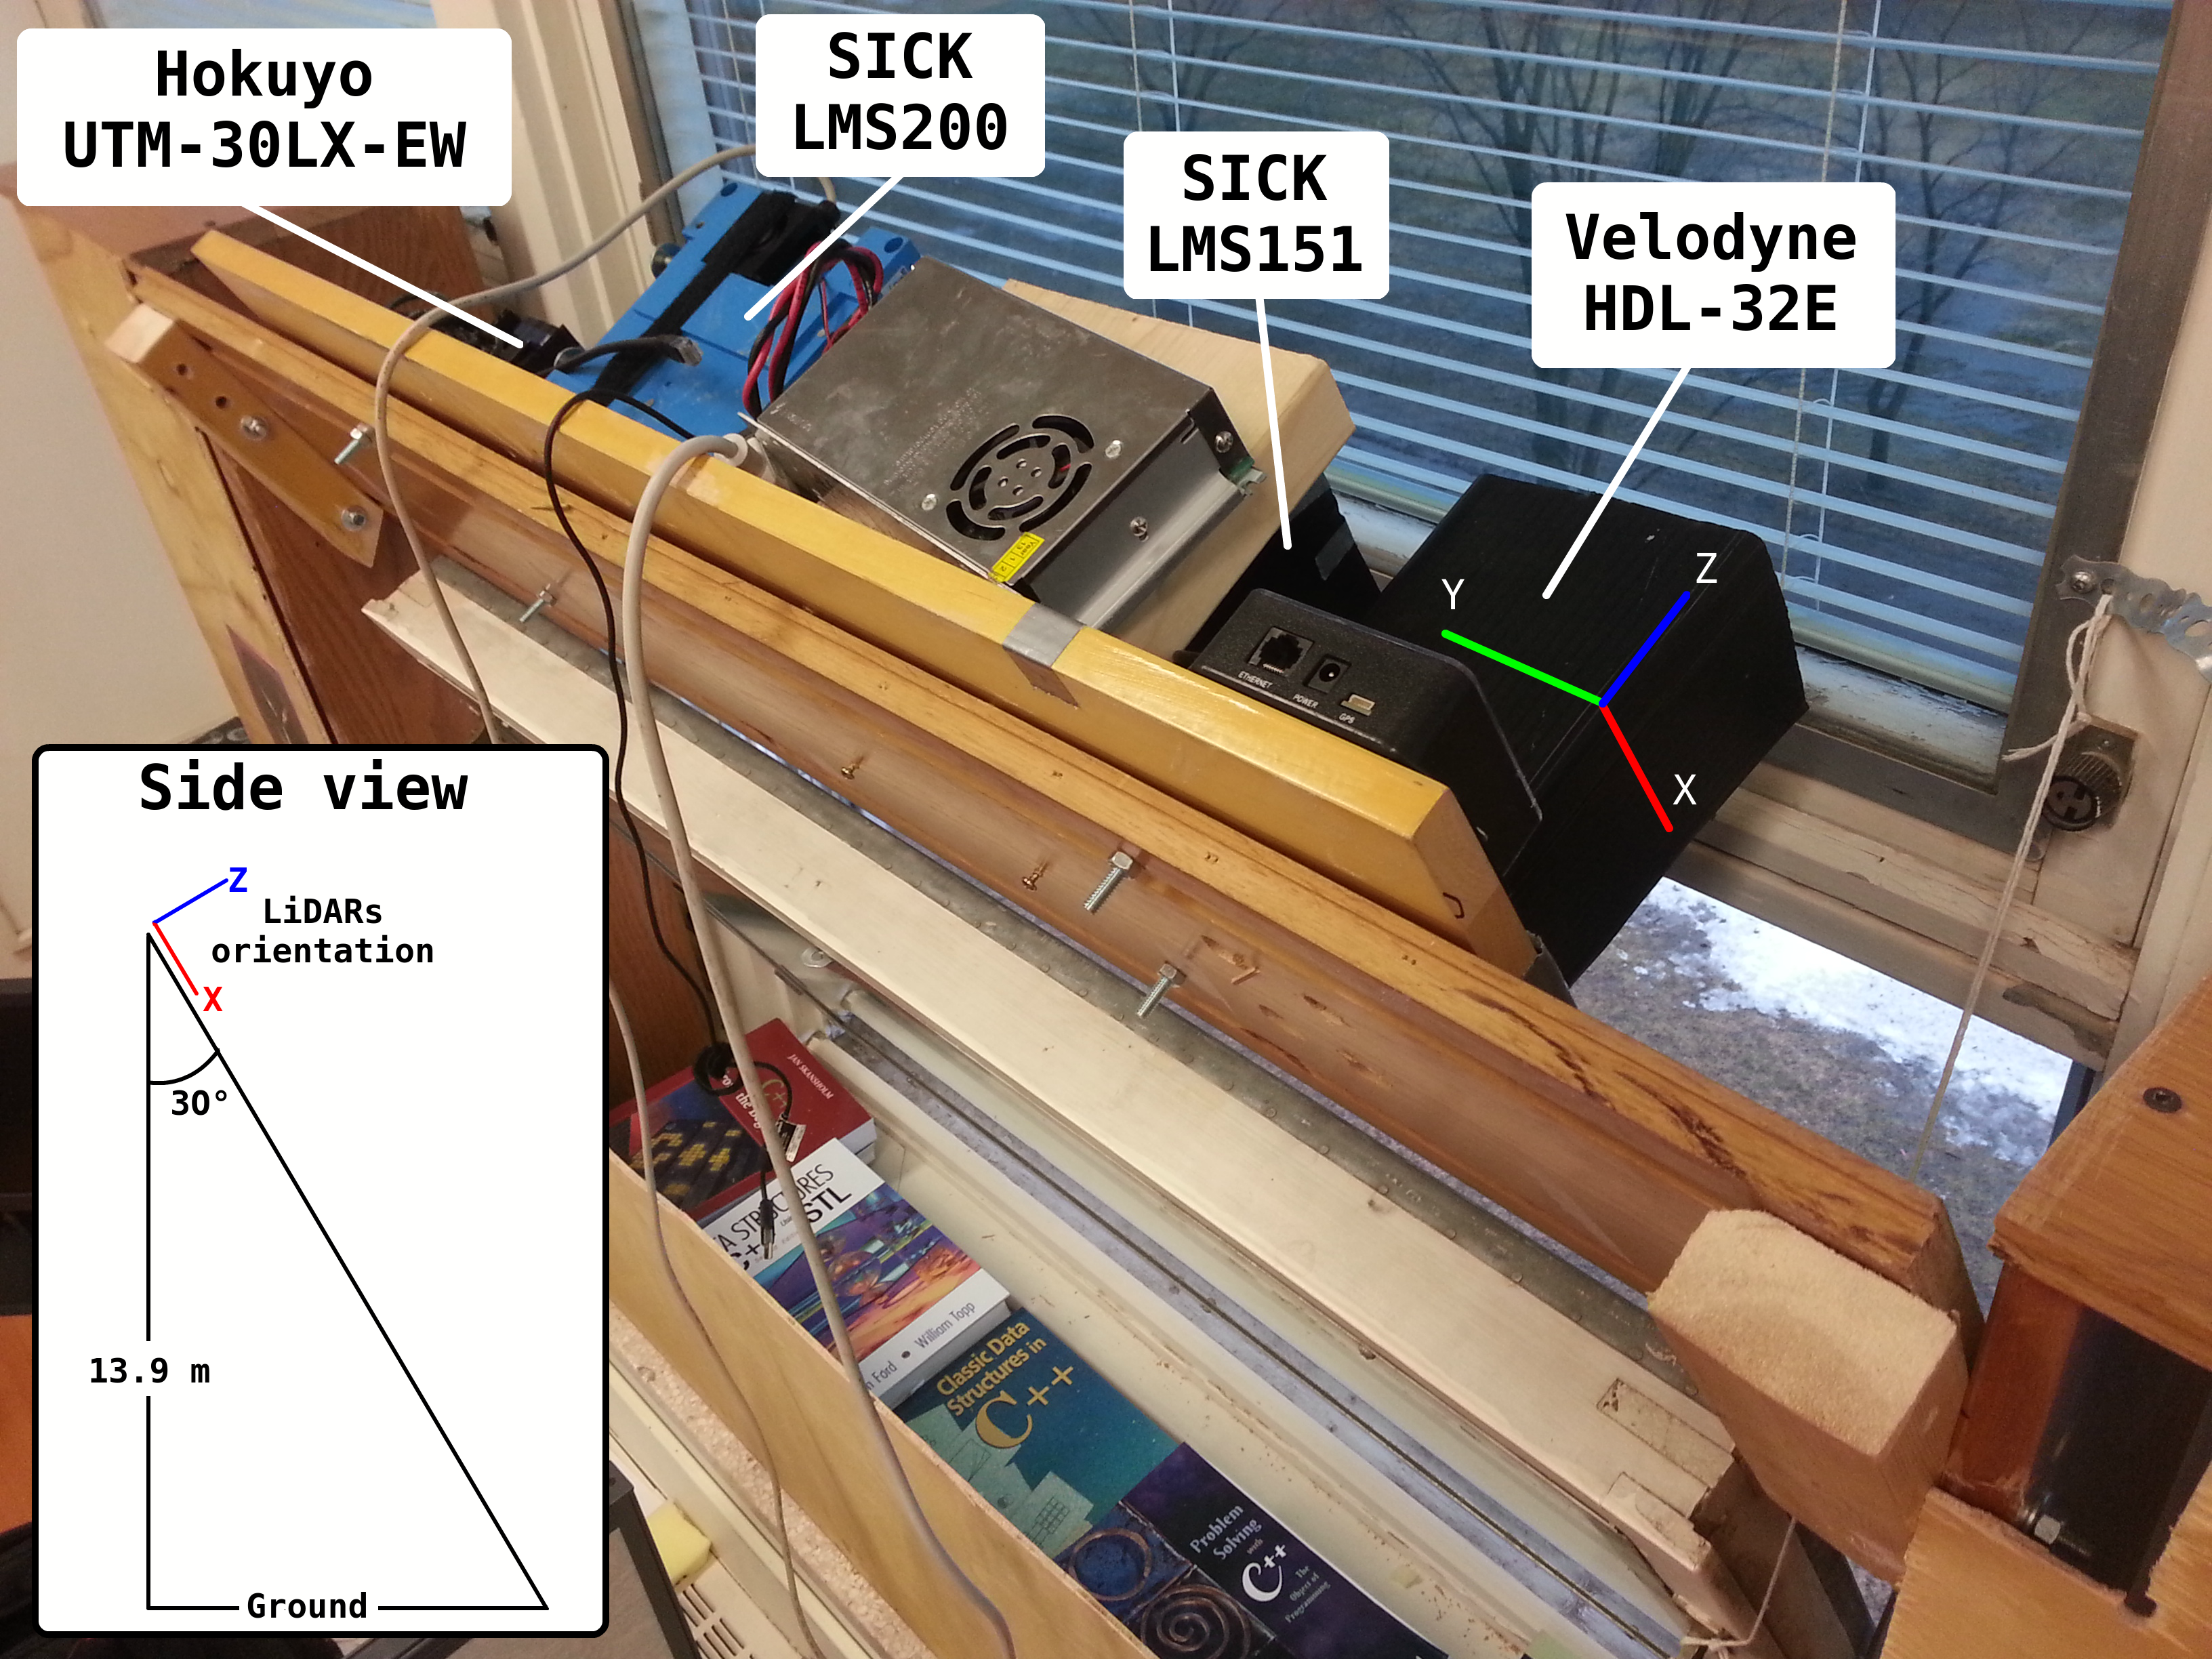
\includegraphics[width=0.95\linewidth]{./img/setup_diag.png}
    \caption{The experimental setup. The 3D axis represent the orientation of the sensors and the bottom left panel represent the 2D geometry as seen from the right side of the picture.}
    \label{fig:setup}
\end{figure}
\begin{figure}[h]
    \centering
    \includegraphics[width=0.90\linewidth]{./img/camera_view.jpg}
    \includegraphics[width=0.95\linewidth]{./img/shadow2.png}
    \caption{View from the RGB camera. The sequence of pictures at the bottom shows the evolution of the shadow caused by the building between 10:00~am and 10:40~am.}
    \label{fig:view}
\end{figure}

\subsection{Dataset Description} % TODO change number of acquisitions and overall time if required (and check abstract also)
Data acquisition started February~11 and ended on March~21. A total of 14 samples were obtained for a total of more than 78 hours of data. Recording was made using the Robot Operating System (ROS)~\cite{ROSWeb}, which provide standardized data type as well as time synchronisation. Data was acquired at different time of the day and in a wide variety of conditions: snowflakes size and falling rate, clear and covered sky, wind speed. The target ground area also changed from different amount and type of snow to complete grass.
